% V0 : 

% !TeX program = pdflatex
% Template modulaire FR pour CV — deux colonnes, personnalisable via commandes en tête

\documentclass[12pt, a4paper]{article}

\usepackage[T1]{fontenc}
\usepackage[utf8]{inputenc}
\usepackage[french]{babel}
\usepackage[left=8mm, right=8mm, top=8mm, bottom=8mm]{geometry}
\usepackage{graphicx}
\usepackage{xcolor}
\usepackage{setspace}

\renewcommand{\familydefault}{\sfdefault}
\linespread{1.05}

\definecolor{cvblue}{HTML}{304263}
\definecolor{cvgold}{HTML}{FFC600}

\usepackage[colorlinks=true, urlcolor=white, linkcolor=white]{hyperref}

\usepackage{fancyhdr}

% --- Personnalisation (modifiez ces commandes avant de compiler) ---
\newcommand{\cvname}{<<CVNAME>>}
\newcommand{\cvaddress}{<<CVADDRESS>>}
\newcommand{\cvmail}{<<CVMAIL>>}
\newcommand{\cvphone}{<<CVPHONE>>}
\newcommand{\cvlinkedin}{<<CVLINKEDIN>>}
\newcommand{\cvgithub}{<<CVGITHUB>>}
\newcommand{\jobtype}{<<JOBTYPE>>}
\newcommand{\presentation}{<<PRESENTATION>>}


% ----- COMMANDES DE MISE EN FORME (style LuxSleek) -----
\newlength{\headleftwidth}
\newcommand{\headleft}[1]{%
    \vspace*{1.5ex}%
    \settowidth{\headleftwidth}{\textsc{\textbf{#1}}}%
    {\color{cvgold}\textsc{\textbf{#1}}}\par%
    \vspace*{-1.5ex}%
    {\color{cvgold}\rule{\headleftwidth}{0.4pt}}%
    \par\vspace*{0.3ex}
}

\newcommand{\headright}[1]{%
  \vspace*{1.5ex}%
  \textsc{\large\color{cvblue}#1}\par%
  \vspace*{-1.5ex}%
  {\color{cvblue}\rule{\headleftwidth}{0.4pt}}%
  \par\vspace*{0.1ex}}

\newcommand{\dates}[1]{\hfill\mbox{\textbf{#1}}}

\newcommand{\is}{\par\vskip.5ex plus .4ex}

\newcommand{\smaller}[1]{{\small$\diamond$\ #1}}

  \begin{document}

  \setlength{\topskip}{0pt}
  \setlength{\parindent}{0pt}
  \setlength{\parskip}{0pt}
  \setlength{\fboxsep}{0pt}
  \raggedbottom

  % ===== COLONNE GAUCHE (sidebar color\'{e}e ~30%) =====
  %\begin{minipage}[t][\textheight]{0.30\textwidth}
  \begin{minipage}[t]{0.30\textwidth}
    \fcolorbox{cvblue!90}{cvblue!90}{\color{white}
      %\kern0.02\textwidth\relax
      \begin{minipage}[t]{0.96\textwidth}
        \raggedright
        \vspace*{2ex}
        % ===== DISPOSITION - COLONNE A GAUCHE | Section INTITULE DE POSTE VISE =====
        \input{sections/intitule_poste.tex}

        \vspace*{2ex}
        % ===== DISPOSITION - COLONNE A GAUCHE | Section Disponibilit\'{e} =====
        \input{sections/disponibilite.tex}

        \vspace*{04ex}
        % ===== DISPOSITION - COLONNE A GAUCHE | Section Atouts =====
        \input{sections/atouts.tex}
        \vspace*{04ex}

        % ===== DISPOSITION - COLONNE A GAUCHE | Section Langues =====
        \input{sections/langues.tex}
        \vspace*{04ex}

        % ===== DISPOSITION - COLONNE A GAUCHE | Section Centre d'int\'{e}r\^{e}t =====
        \input{sections/centre_interet.tex}

        \vspace*{04ex}
        % ===== DISPOSITION - COLONNE A GAUCHE | Section Photo profil =====
        \null\hfill
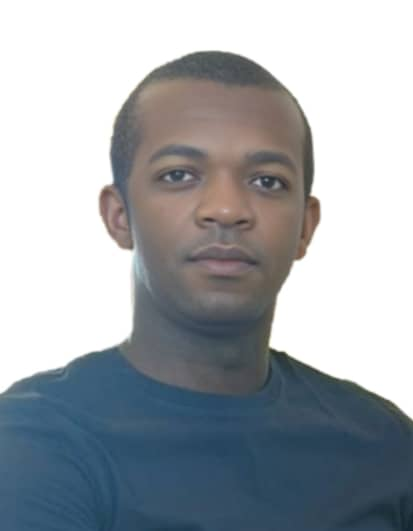
\includegraphics[width=0.65\textwidth]{../pictures/photo_cv.jpg}
\hfill\null
\vspace*{0.5ex}


        % ===== DISPOSITION - COLONNE A GAUCHE | Section En-t\^{e}te =====
        % Header: utilise les commandes definies dans main.tex
\begin{center}
    {\Large \textbf{\cvname}}\\[3pt]
    {\small \cvaddress{} \quad$\cdot$\quad \href{mailto:\cvmail}{\cvmail} \quad$\cdot$\quad
    Tél : \cvphone}\\[3pt]
    \href{https://linkedin.com/in/\cvlinkedin}{\faLinkedinIn\ \cvlinkedin} \quad$\cdot$\quad
    \href{https://github.com/\cvgithub}{\faGithub\ \cvgithub}
\end{center}

\vspace{0.2cm}


        \vspace*{01ex}
        % ===== DISPOSITION - COLONNE A GAUCHE | Section Informations =====
        \input{sections/informations.tex}

      \end{minipage}
      \kern0.02\textwidth\relax
    }
  \end{minipage}


  % ===== COLONNE DROITE (contenu principal ~70%) =====
  \hskip0.01\textwidth%
  %\begin{minipage}[t][\textheight]{0.695\textwidth}
  \begin{minipage}[t]{0.695\textwidth}
    \setlength{\parskip}{0.1ex}
    \vspace{02ex}

    % ===== DISPOSITION - COLONNE A DROITE | Section Exp\'{e}riences professionnelles =====
    % Exemples d'entrées — remplacez par vos expériences réelles
\textbf{Alternant Data Analyst – NaTran France (Spécialiste national des données gazières)} \hfill \textit{Septembre 2023 – Présent}\\
\textit{Ingénierie de la données, Département Data}
\begin{itemize}
    \item Développement de tableaux de bord nationaux sous \textbf{Power BI}, intégrant des jeux de données hétérogènes et réduisant le temps de reporting de 40\%.
    \item Conception et optimisation de pipelines de traitement de données avec \textbf{Python (Pandas, PySpark)}, automatisant des tâches récurrentes.
\end{itemize}

% Ajoutez d'autres expériences au besoin

    \vspace*{04ex}

    % ===== DISPOSITION - COLONNE A DROITE | Section Projets académiques =====
    \input{sections/projets.tex}
    \vspace*{05ex}

    % ===== DISPOSITION - COLONNE A DROITE | Section Compétences techniques =====
    \input{sections/competences_techniques.tex}
    \vspace*{05ex}

    % ===== DISPOSITION - COLONNE A DROITE | Section Formations =====
    \input{sections/formations.tex}

    % ===== DISPOSITION - COLONNE A DROITE | Section Certifications =====
    % Certifications — listez vos certifications ici
\begin{itemize}
    \item Microsoft Certified: Data Analyst Associate (en cours) – Power BI
    \item Bloomberg Market Concepts (BMC) (en cours)
    \item Certification AMF (en cours)
\end{itemize}


  \end{minipage}

\end{document}


% ==========================================

%V1 : 

% !TeX program = pdflatex
% Template modulaire FR pour CV — deux colonnes, personnalisable via commandes en tête

\documentclass[12pt, a4paper]{article}

\usepackage[T1]{fontenc}
\usepackage[utf8]{inputenc}
\usepackage[french]{babel}
\usepackage[left=4mm, right=4mm, top=4mm, bottom=4mm]{geometry}
\usepackage{graphicx}
\usepackage{xcolor}
\usepackage{setspace}
\usepackage{paracol}
\usepackage{tcolorbox}

\renewcommand{\familydefault}{\sfdefault}
\linespread{1.05}

\definecolor{cvblue}{HTML}{304263}
\definecolor{cvgold}{HTML}{FFC600}

\usepackage[colorlinks=true, urlcolor=white, linkcolor=white]{hyperref}

\usepackage{fancyhdr}

% --- Personnalisation ---
\newcommand{\cvname}{<<CVNAME>>}
\newcommand{\cvaddress}{<<CVADDRESS>>}
\newcommand{\cvmail}{<<CVMAIL>>}
\newcommand{\cvphone}{<<CVPHONE>>}
\newcommand{\cvlinkedin}{<<CVLINKEDIN>>}
\newcommand{\cvgithub}{<<CVGITHUB>>}
\newcommand{\jobtype}{<<JOBTYPE>>}
\newcommand{\presentation}{<<PRESENTATION>>}

% ----- STYLE -----
\newlength{\headleftwidth}
\newcommand{\headleft}[1]{%
    \vspace*{1.5ex}%
    \settowidth{\headleftwidth}{\textsc{\textbf{#1}}}%
    {\color{cvgold}\textsc{\textbf{#1}}}\par%
    \vspace*{-1.5ex}%
    {\color{cvgold}\rule{\headleftwidth}{0.4pt}}%
    \par\vspace*{0.3ex}
}

\newcommand{\headright}[1]{%
  \vspace*{1.5ex}%
  \textsc{\large\color{cvblue}#1}\par%
  \vspace*{-1.5ex}%
  {\color{cvblue}\rule{\headleftwidth}{0.4pt}}%
  \par\vspace*{0.1ex}}

\newcommand{\dates}[1]{\hfill\mbox{\textbf{#1}}}
\newcommand{\is}{\par\vskip.5ex plus .4ex}
\newcommand{\smaller}[1]{{\small$\diamond$\ #1}}

\begin{document}

  \setlength{\topskip}{0pt}
  \setlength{\parindent}{0pt}
  \setlength{\parskip}{0pt}
  \setlength{\fboxsep}{0pt}
  \raggedbottom

  % ===== STRUCTURE PARACOL =====
  \columnratio{0.30,0.70}
  \begin{paracol}{2}

    % ===== COLONNE GAUCHE =====
    \switchcolumn[0]

    \begin{tcolorbox}[
      colback=cvblue!90,
      colframe=cvblue!90,
      coltext=white,
      boxrule=0pt,
      arc=0pt,
      left=4pt,right=4pt,top=4pt,bottom=4pt,
      height=\textheight
    ]

    \raggedright
    \vspace*{1ex}

    \input{sections/intitule_poste.tex}
    \vspace*{1ex}

    \input{sections/disponibilite.tex}
    \vspace*{2ex}

    \input{sections/atouts.tex}
      \vspace*{2ex}

      \input{sections/langues.tex}
      \vspace*{2ex}

      \input{sections/centre_interet.tex}
      \vspace*{2ex}

      \null\hfill
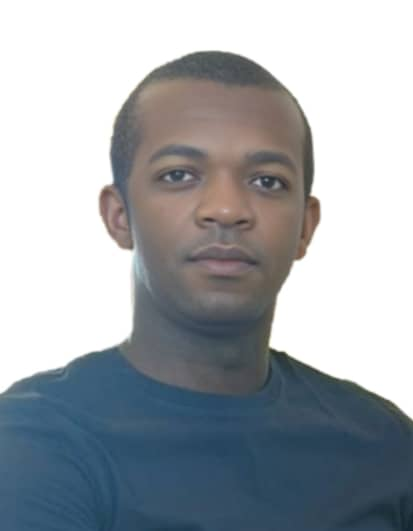
\includegraphics[width=0.65\textwidth]{../pictures/photo_cv.jpg}
\hfill\null
\vspace*{0.5ex}


      % Header: utilise les commandes definies dans main.tex
\begin{center}
    {\Large \textbf{\cvname}}\\[3pt]
    {\small \cvaddress{} \quad$\cdot$\quad \href{mailto:\cvmail}{\cvmail} \quad$\cdot$\quad
    Tél : \cvphone}\\[3pt]
    \href{https://linkedin.com/in/\cvlinkedin}{\faLinkedinIn\ \cvlinkedin} \quad$\cdot$\quad
    \href{https://github.com/\cvgithub}{\faGithub\ \cvgithub}
\end{center}

\vspace{0.2cm}

      \vspace*{1ex}

      \input{sections/informations.tex}

      \end{tcolorbox}

    % ===== COLONNE DROITE =====
    \switchcolumn

    \setlength{\parskip}{0.1ex}
    \vspace{1ex}

    % Exemples d'entrées — remplacez par vos expériences réelles
\textbf{Alternant Data Analyst – NaTran France (Spécialiste national des données gazières)} \hfill \textit{Septembre 2023 – Présent}\\
\textit{Ingénierie de la données, Département Data}
\begin{itemize}
    \item Développement de tableaux de bord nationaux sous \textbf{Power BI}, intégrant des jeux de données hétérogènes et réduisant le temps de reporting de 40\%.
    \item Conception et optimisation de pipelines de traitement de données avec \textbf{Python (Pandas, PySpark)}, automatisant des tâches récurrentes.
\end{itemize}

% Ajoutez d'autres expériences au besoin

    \vspace*{2ex}

    \input{sections/projets.tex}
    \vspace*{2ex}

    \input{sections/competences_techniques.tex}
    \vspace*{2ex}

    \input{sections/formations.tex}

    % Certifications — listez vos certifications ici
\begin{itemize}
    \item Microsoft Certified: Data Analyst Associate (en cours) – Power BI
    \item Bloomberg Market Concepts (BMC) (en cours)
    \item Certification AMF (en cours)
\end{itemize}


  \end{paracol}

\end{document}









